\section{绪论}
\subsection{研究背景}
泰坦尼克号是英国白星航运公司20世纪10年代建设的一搜豪华游艇。其排水量达到了惊人的4.6万吨,是当时世界上体积最大,最豪华的客运轮船。但正是这艘号称“永不沉没”的泰坦尼克号,在1912年从英国驶往美国时,在大西洋与冰山相撞并沉没!

根据英国贸易委员会公布的数据显示,在灾难发生时,泰坦尼克号共搭载2224人,其中710人生还,1514人不幸罹难,其中乘客约有1317人,共498人幸存;男性船员约有885人,共192人幸存;女性船员23人,共20人幸存。


\textbf{大数据比赛}是一项综合Python编程,数据分析,机器学习的比赛。常见的大数据比赛包括Kaggle比赛,“钉钉杯”大数据挑战赛,微信大数据挑战赛。大数据比赛一般流程包括数据初步探索,数据可视化探索,特征工程,模型建立与验证,模型调参,模型融合等。
\subsection{研究内容}
本课程设计的\textbf{研究内容}就是使用数据分析比赛的流程对泰坦尼克号幸存者的数据进行分析,提取有效信息,得出有效结论;并在数据分析的基础上,建立预测模型,对测试集的数据进行预测。

\subsection{研究目的}
本课程设计的\textbf{研究目的}就是通过对泰坦尼克号的数据分析和模型建立,从而熟练掌握jupyterlab,anaconda,Python常用包的使用和方法;深刻理解数据分析,机器学习的步骤和算法。

\subsection{研究思路}
本课程设计第一步在导入数据后进行数据的初步探索,包括查看数据的基本属性,缺失值数据,统计数据,每个属性的基本信息;第二步通过数据可视化,进一步探索属性与属性之间关系并提取有效信息,得出有效结论,为特征工程做准备;第三步进行特征工程,包括数据预处理,缺失值处理,模型训练和模型验证;第四步使用网格搜索思想对模型参数进行优化;第五步使用Stacking对模型进行融合。
\clearpage
具体研究思路如下:



\begin{figure}[htbp]
	\centering
	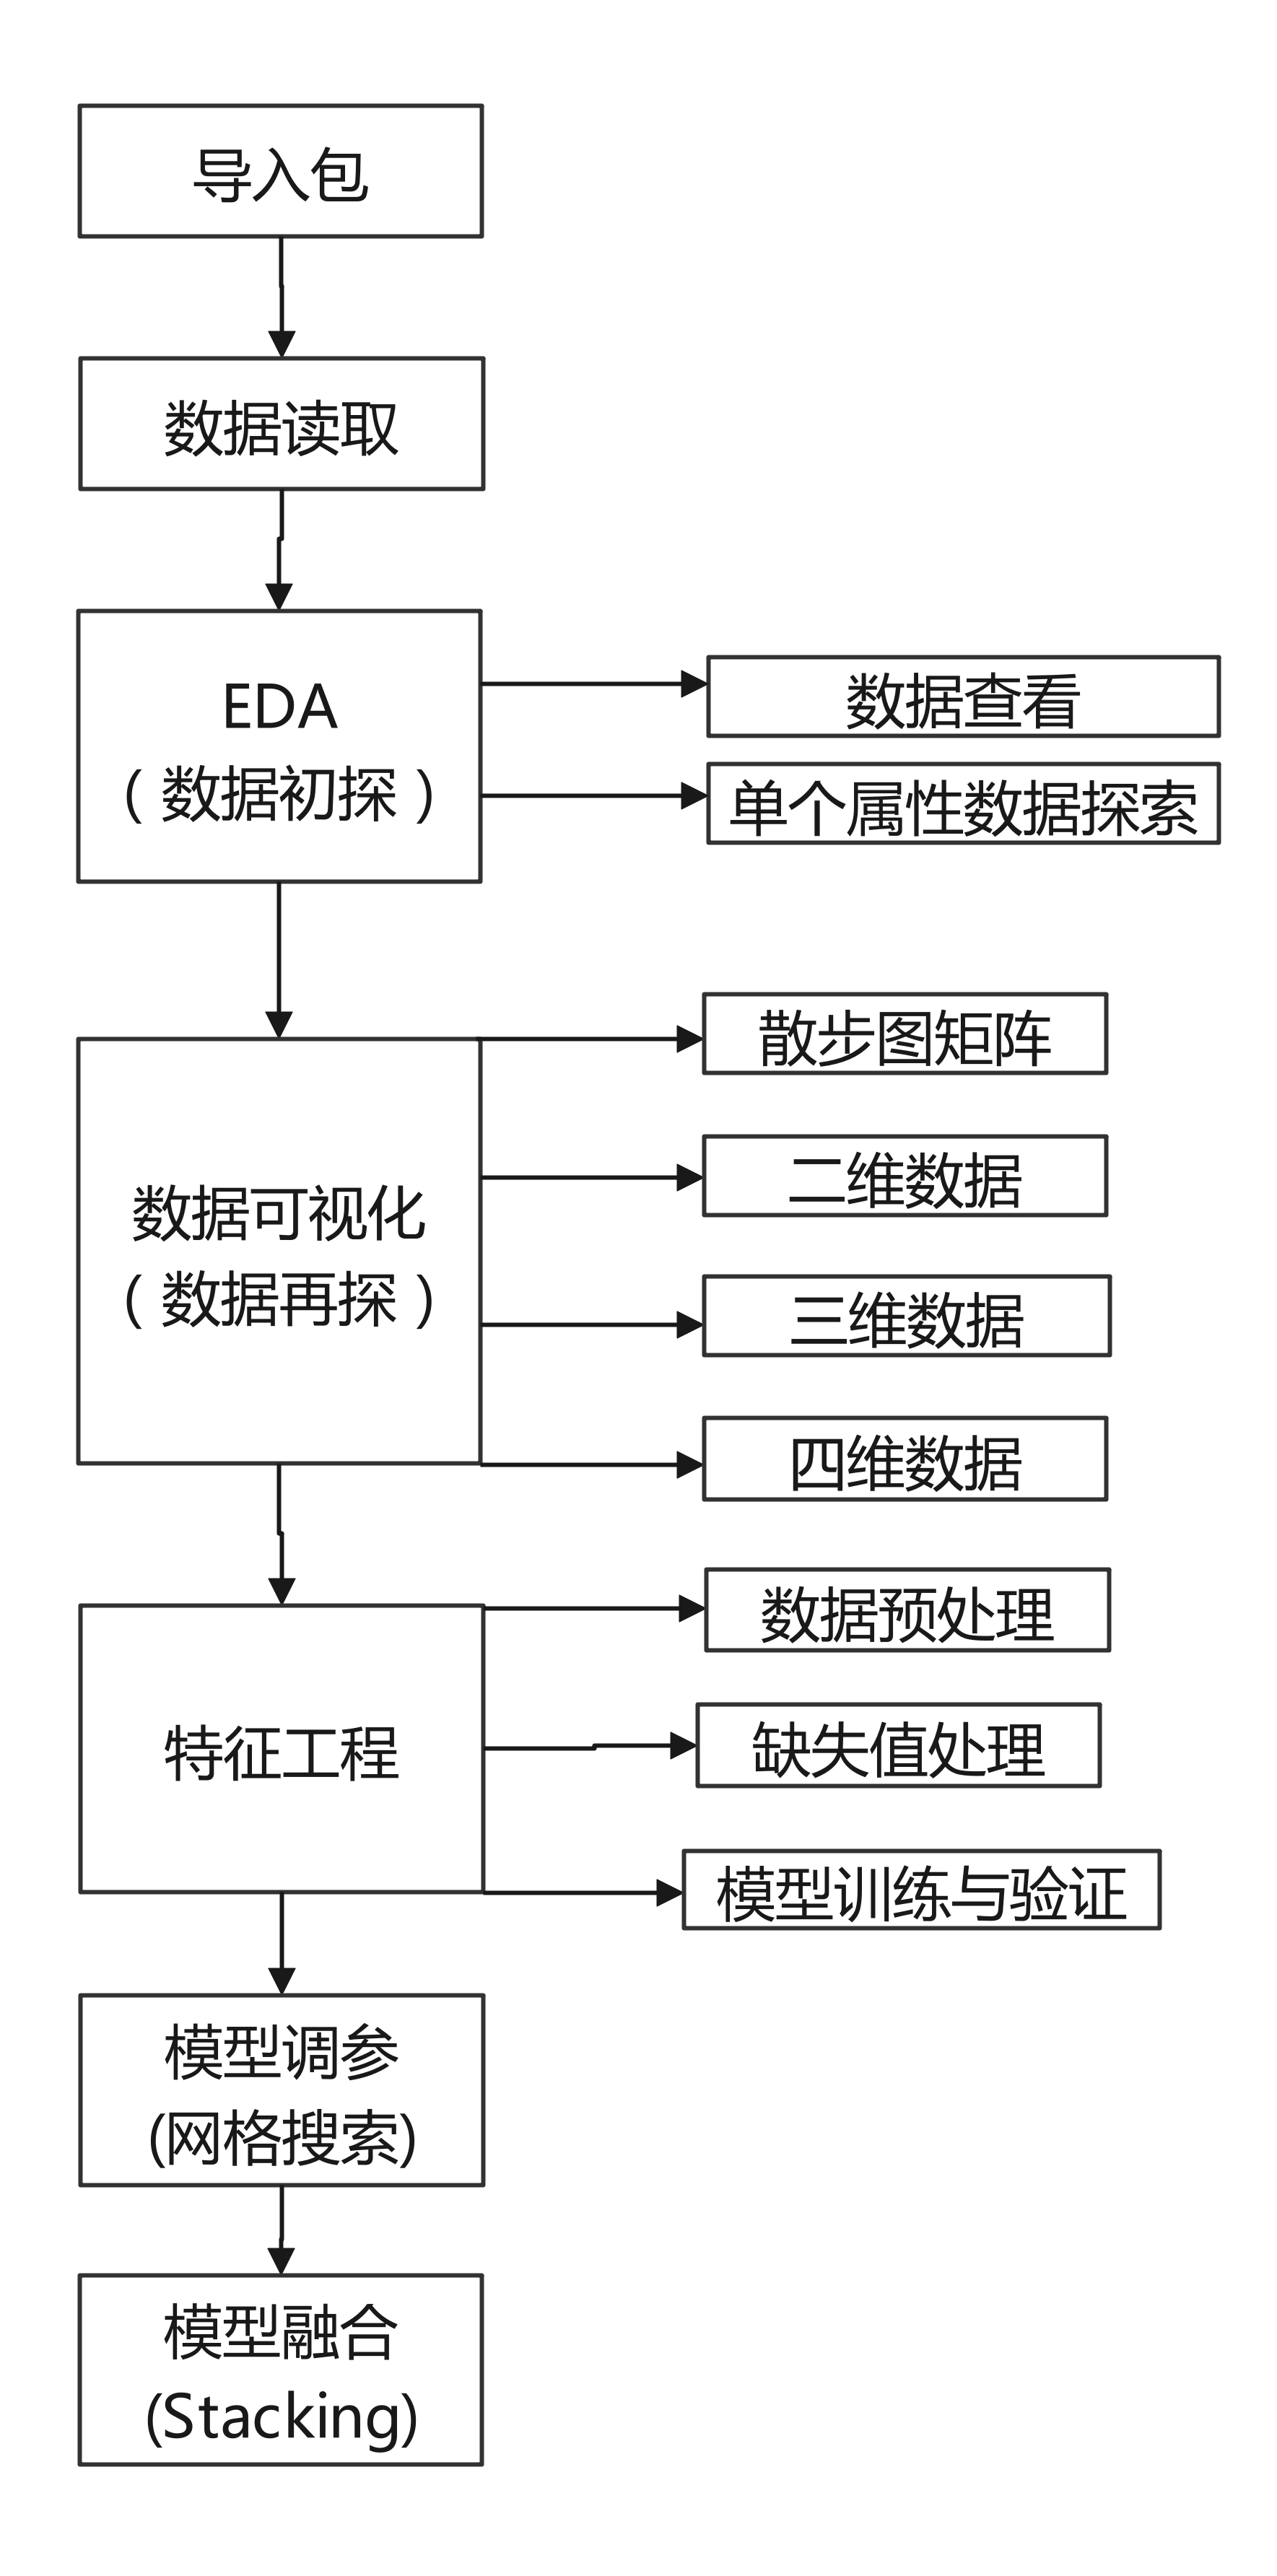
\includegraphics[scale=0.1,angle=0]{images/1.png}
	\caption{论文研究思路}
	\label{1}
\end{figure}


\section{EDA(数据初探)}
\subsection{导入包}
		\begin{figure}[H]
			\centering
			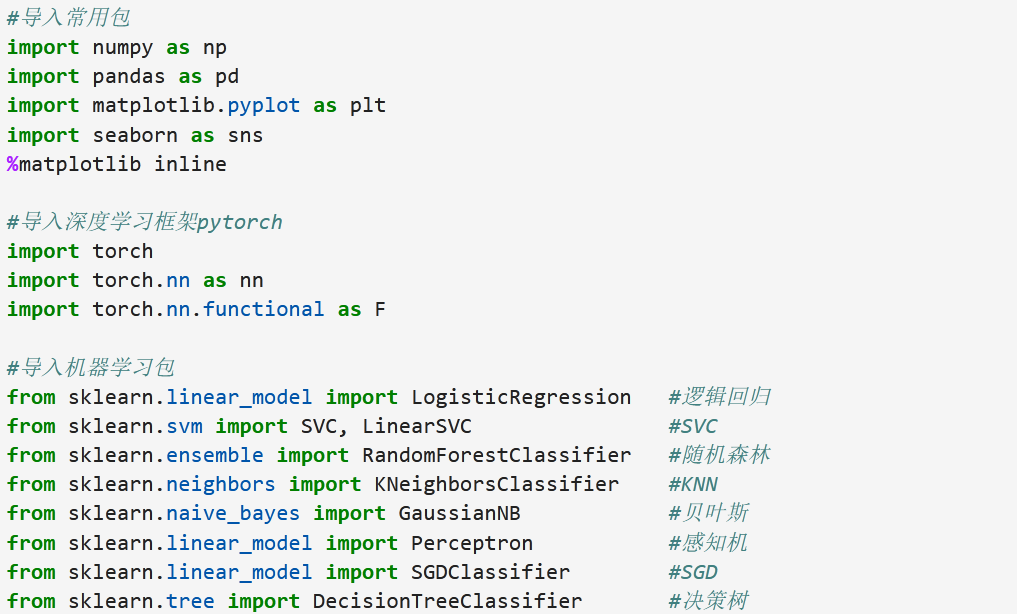
\includegraphics[scale=0.40,angle=0]{images/2.png}
			\caption{导入常用的包}
			\label{2}
		\end{figure}
首先导入本课程设计需要的包,其中常用包包括了numpy,pandas,matplotlib,seaborn;pytorch是一个深度学习框架,本文中用于对缺失数据Age的预测填充;scikit-learn的包包括了逻辑回归,SVC,随机森林,KNN,朴素贝叶斯,感知机,SGD和决策树,本文中用于训练并预测泰坦尼克号乘客的幸存与否。

\subsection{数据读取}
\begin{figure}[H]
	\centering
	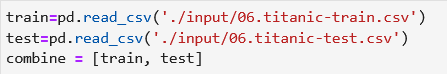
\includegraphics[scale=1.0,angle=0]{images/3.png}
	\caption{读取训练集和测试集}
	\label{3}
\end{figure}
分别读取数据集和测试集,其中conbine将train和test合并,便于查看数据和处理数据。
		
\subsection{查看数据}
首先查看数据,包括数据的行数列数,训练集前5行,基本信息,缺失值和统计数据。其中基本信息如图\ref{4},其他数据信息见附录3.3.1。
	\begin{figure}[H]
		\centering
		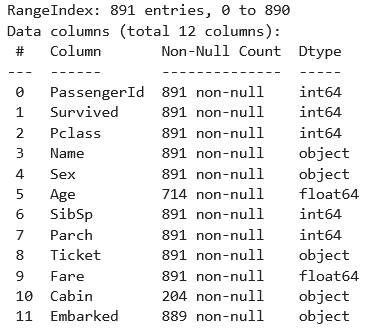
\includegraphics[scale=0.8,angle=0]{images/4.png}
		\caption{训练集基本信息}
		\label{4}
	\end{figure}
训练集共有891行;训练集包含12个属性,分别为乘客Id,是否幸存,客舱等级,姓名,性别,年龄,同代亲属数,不同代亲属数,船票编号,床票价格,客舱号,登船港口;其中Age缺失177个数据,Cabin缺失687个数据,Embarked缺失两个数据;通过查看统计信息,没有发现异常值。
\subsection{单个属性数据探索}
对训练集Survived,Pclass,Sex,Age,SibSp,Parch,Fare,Embarked共8个属性进行计数并绘制直方图,可以提取以下信息:
\begin{itemize}
	\item 幸存者342人,遇难549人,幸存者比例为 $38.38 \%$;
	\item 三等仓人数最多,为55.1\%,一等舱为24.2\%,二等舱20.7\%;
	\item 男性577人,女性314人,男性更多,占64.76\%;
	\item  20岁-40岁的人较多 ;
	\item 68\%的人没有同级亲属,23\%的人有一个同级亲属,同级亲属有两个以上的很少;
	\item 76.1\%的人没有非同级亲属,13\%的人有一个非同级亲属 ;
	\item 大部分的船票在100美元以下 ;
	\item 72\%的人从S上船,18\%从C上船,只有8\%的人从Q上船。
\end{itemize}
其中,对Survived的探索结果如图\ref{5},Pclass,Sex,Age,SibSp,Parch,Fare,Embarked的探索结果见附录3.3.2。
\begin{figure}[H]
	\centering
	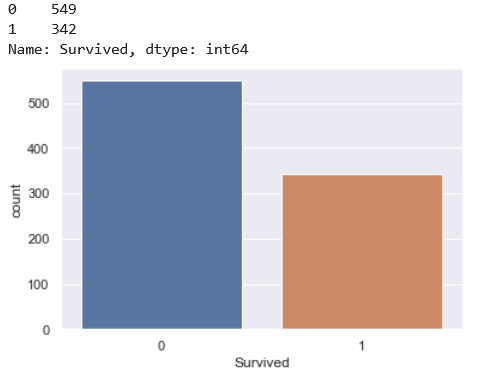
\includegraphics[scale=0.8,angle=0]{images/5.png}
	\caption{对单属性Survived的探索结果}
	\label{5}
\end{figure}

\clearpage

\section{数据可视化(数据再探)}
	\subsection{数据总体概览}
	通过绘制散布图矩阵,查看所有数据的整体情况。如下图所示:
		\begin{figure}[H]
			\centering
			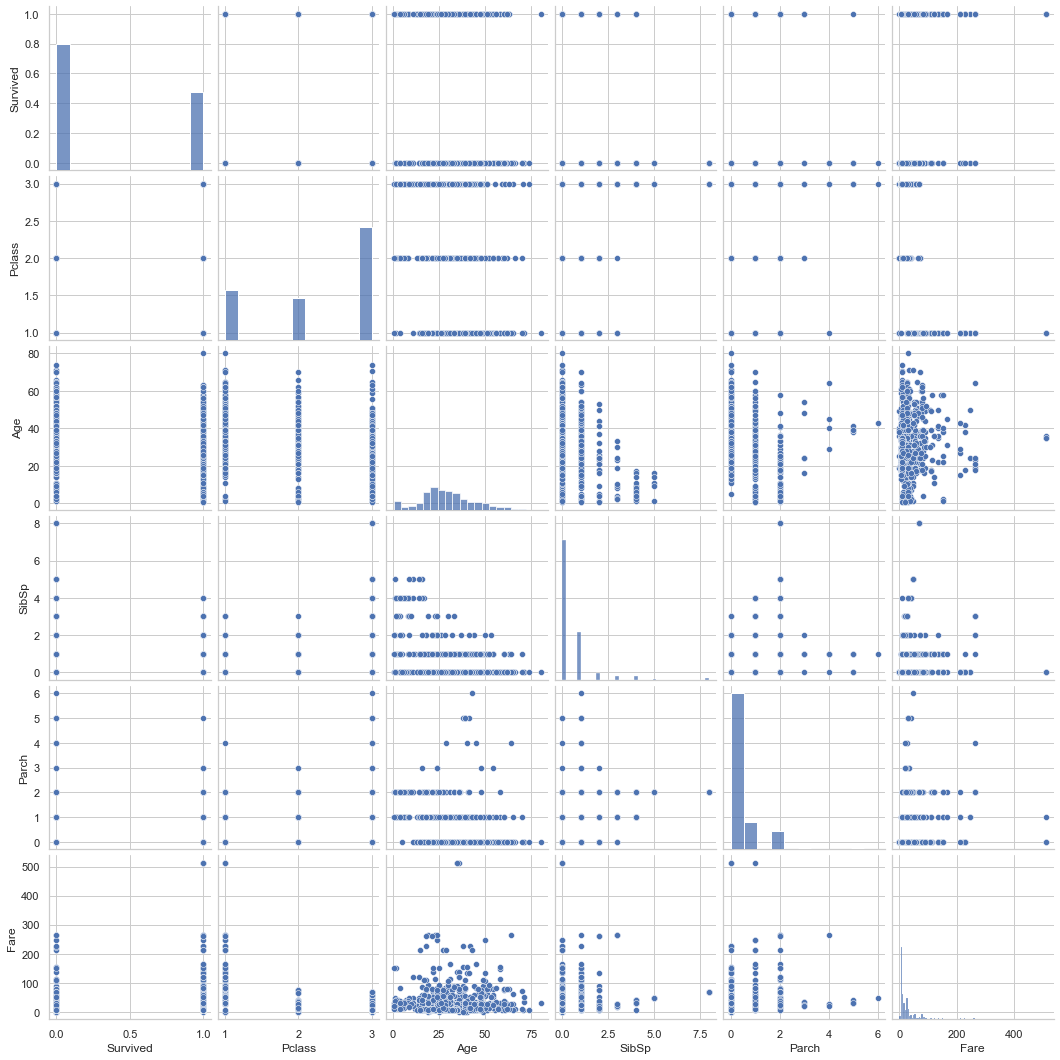
\includegraphics[scale=0.3,angle=0]{images/6.png}
			\caption{训练集散布图矩阵}
			\label{6}
		\end{figure}
其中散步图的矩阵的对角线位置在2.4中已经进行了阐述,下面进行非对角线数据的探索。
\subsection{二维数据探索}
	通过绘制Fare 与 Pclass,Sex 与 Pclass,Pclass 与 Survived,Sex 与 Survived,Age 与 Survived,SibSp 与 Survived,Parch 与 Survived,Fare 与 Survived,Embarked 与 Survived的散点图或者计数图,可得以下结论:

\begin{itemize}
	\item 费用与船舱等级具有较高的相关性,费用越多,船舱等级可能越高,比尔森系数为-0.55;
	\item 各个船舱,男性乘客均多余女性乘客;
	\item 一等舱的幸存率最高,三等舱幸存率最低,幸存率与船舱有重要关系;
	\item  女性的生存率为74.2\%,远高于男性的18.9\%,性别与生存与否具有重要关系;
	\item 孩子和老人的生存率明显高于死亡率,而成年的死亡率明显高于生存率,年龄与生存与否具有重要关系;
	\item 船费更高的倾向于更高的的生存率。
\end{itemize}
其中Sex 与 Survived计数图,Age 与 Survived的条形图如\ref{7}所示,其他的二维数据图见附录3.4.2。
		\begin{figure}[H]
	\centering
	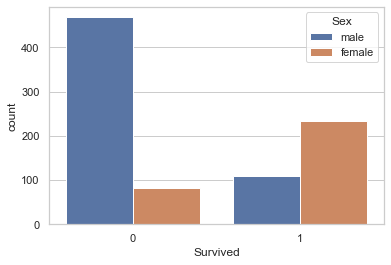
\includegraphics[scale=0.5,angle=0]{images/7.png}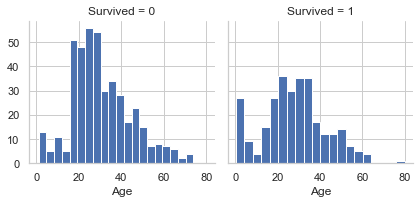
\includegraphics[scale=0.65,angle=0]{images/8.png}
	\caption{Sex 与 Survived计数图,Age 与 Survived的条形图}
	\label{7}
\end{figure}	

\subsection{三维数据探索}
通过绘制Sex 与 Survived,Pclass;Age 与 Survived,Pclass;SibSp 与 Survived,Pclass;Parch 与 Survived,Pclass;Embarked 与 Survived,Pclass的计数分布条形图,可以得到以下结论:
\begin{itemize}
	\item 各个等级船舱,女性生存率高于男性; 高等级船舱生存率更高;
	\item 船舱一,死亡数较少;船舱二,死亡数中等;船舱三,孩子死亡少,成年死亡多
\end{itemize}	
其中Sex 与 Survived,Pclass、Age 与 Survived,Pclass如图\ref{9}:其他三维数据见附录3.4.3

\clearpage


\begin{figure}[H]
	\centering
	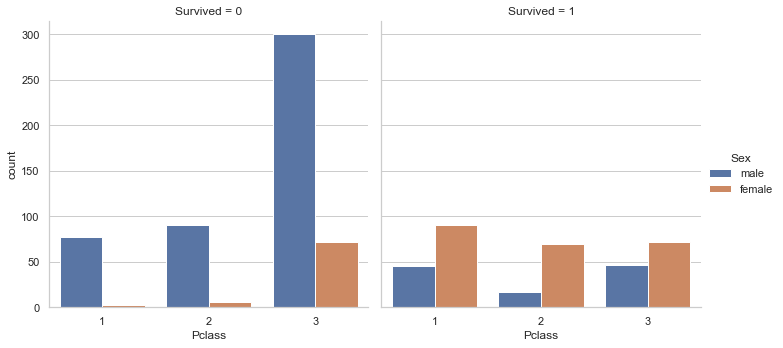
\includegraphics[scale=0.34,angle=0]{images/9.png}	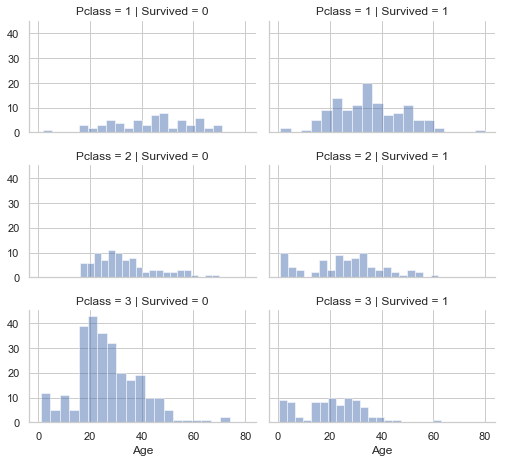
\includegraphics[scale=0.34,angle=0]{images/10.png}

	\caption{Sex 与 Survived,Pclass及Age 与 Survived,Pclass计数分布条形图}
	\label{9}
\end{figure}

\subsection{四维数据探索}
通过绘制Embarked,Sex,Pclass 与 Survived、Fare,Sex,Embarked 与 Survived计数分布条形图如下:
\begin{figure}[H]
	\centering
	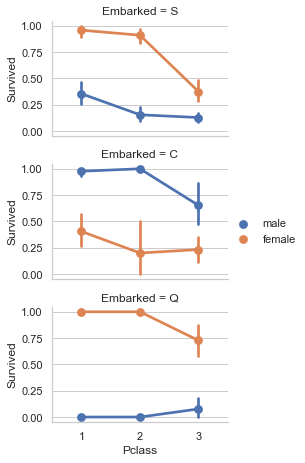
\includegraphics[scale=0.5,angle=0]{images/11.png}	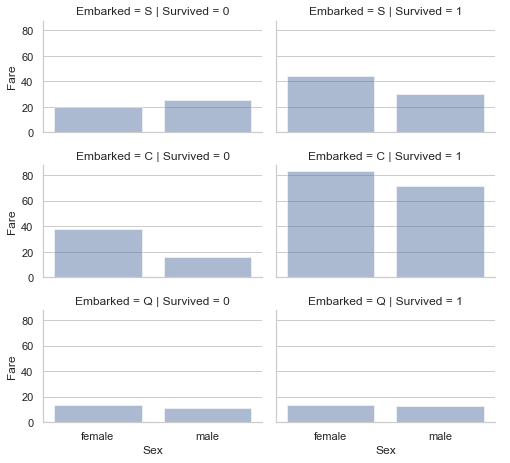
\includegraphics[scale=0.5,angle=0]{images/12.png}
	\caption{Embarked,Sex,Pclass 与 Survived及Fare,Sex,Embarked 与 Survived计数分布条形图}
	\label{11}
\end{figure}
	从Embarked,Sex,Pclass 与 Survived计数分布条形图中可以看出Q上岸的人,女性生存率高于男性;一等舱,二等舱的生存率比三等舱高相关性较弱;从Fare,Sex,Embarked 与 Survived计数分布条形图中可以看出幸存的人倾向于更高的船费;Q 上岸的人倾向于更高的船费;男性倾向于更高的船费。
\clearpage
\section{特征工程}
\subsection{数据预处理}
\textbf{(1)剔除无用数据}~~~~ticket,PassengerId 信息无用,cabin 缺失值过多,将二者剔除

\textbf{(2)Sex装换为值}~~~~Sex是一个字符串型的数据,对其进行编码,男性赋值为0.5,女性赋值为-0.5。

\textbf{(3)Embarked缺失值填充并装换为值}~~~~考虑到 Embarked 只缺失了两个数据,通过查找相似数据的众数,确定$C$作为缺失数据的填充值,C赋值为-0.4,S赋值为0.1,Q赋值为0.6

\textbf{(4)合并相似属性}~~~~SibSp 与 Parch 表示的都是亲属,将其合并,建立新属性$family$,表示亲戚的数量。三者的关系为:
$$family=SibSp+Parch+1$$

\textbf{(5)提取Name的有效信息}~~~~Name中包含了特定的称呼,称呼反映了乘客的性别,年龄,职业等信息。首先提取Name中的称呼并进行计数,发现99\%的称呼为Miss,Mr ,Mrs,Master。因此将称呼分为以下五类并进行赋值:
$$"Mr"=1, "Miss"= 2, "Mrs"= 3, "Master"= 4, "other"= 5$$
\subsection{缺失值处理}
\subsection{Fare 的填充及其归一化}
\textbf{(1)填充缺失数据}~~~~测试集中的Fare缺失一个数据,使用中位数对其填充。

\textbf{(2)归一化}~~~~对数据进行归一化,公式如下:
$$x_i=\frac{x_i-x_{min}}{x_{max}-x_{min}}$$
\subsection{age 的预测填充及其归一化}
age中缺失的数据较多,因此考虑建立神经网络对其进行训练和预测。提取训练集和测试集中age非缺失的数据作为训练集,缺失数据作为预测集。神经网络输入包括Pclass,Sex,Age,family,Fare,Embarked,输出为Age,搭建的神经网络及数据集划分见附录3.5.2,对数据进行训练和预测。
\begin{figure}[H]
	\centering
	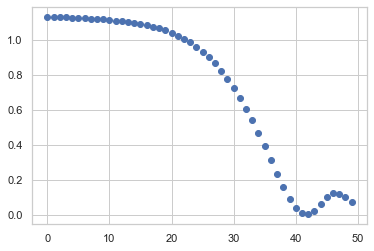
\includegraphics[scale=0.5,angle=0]{images/13.png}	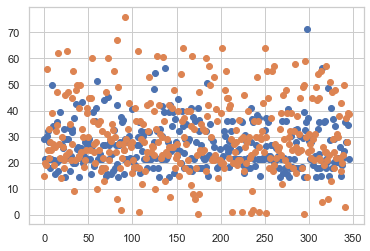
\includegraphics[scale=0.5,angle=0]{images/14.png}
	\caption{损失值变化及在测试集上的效果}
	\label{13}
\end{figure}
从图中可以看出,损失值随着训练次数的增多而逐渐下降。神经网络在测试集上的预测效果相比真实数据相对集中,可以认为神经网络预测效果良好。
\subsection{模型训练与模型验证}
选用逻辑回归,SVC,随机森林,KNN,朴素贝叶斯,感知机,SGD和决策树9种算法,使用训练集的前700个数据作为训练样本,剩余数据作为测试样本,9个模型在测试集上的得分如图\ref{15},模型代码见附录3.5.3。
\begin{figure}[H]
	\centering
	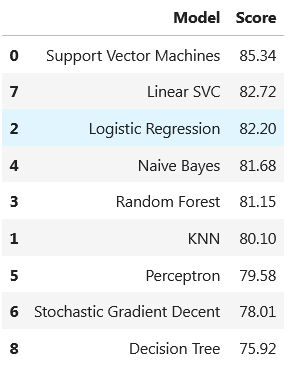
\includegraphics[scale=0.75,angle=0]{images/15.png}
	\caption{各个模型得分情况}
	\label{15}
\end{figure}

从结果可以看出,支持向量机的得分最高,准确率为85.34\%


\section{模型调参 (网格搜索)}
选用随机森林,KNN,决策树,支持向量机等受参数影响较大的模型,通过网格搜索的思想对其进行优化。最终优化结果如图\ref{16},代码见附录3.6。
\begin{figure}[H]
	\centering
	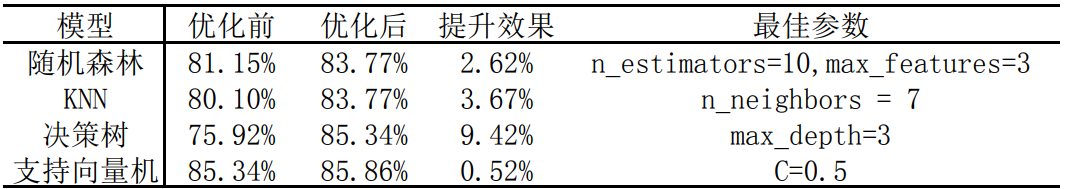
\includegraphics[scale=0.5,angle=0]{images/16.png}
	\caption{参数优化情况情况}
	\label{16}
\end{figure}

\section{模型融合 (Stacking)}
选用随机森林,KNN,决策树,支持向量机,逻辑回归并使用最优参数搭建Stacking模型,Stacking模型的示意图如下:


\begin{figure}[H]
	\centering
	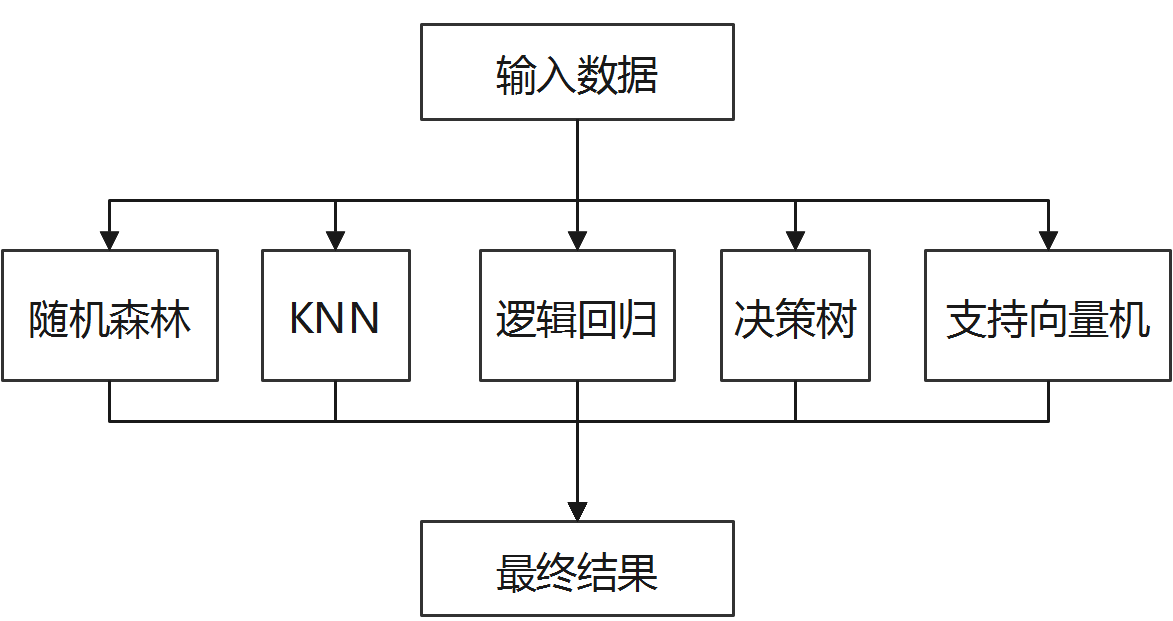
\includegraphics[scale=0.3,angle=0]{images/17.png}
	\caption{Stacking模型}
	\label{17}
\end{figure}
使用Stacking对模型进行融合的准确率为85.86\%。最终使用Stacking模型对测试集进行预测,得出测试集上乘客的幸存与否,提交结果。
\section{结论}
根据数据分析以及模型的预测效果,可以发现在泰坦尼克号乘船事故中,女性、孩子和老人的生还率远远大于男性和成年。一等舱的生还率大于二等舱和三等舱。根据查阅资料显示,在泰坦尼克号发生事故后,船上首先进行了妇孺的疏散,因此妇孺具有更大的机会幸存,本文的分析结果与实际情况相同。

本文通过数据分析与机器学习算法,对泰坦尼克号数据进行数据预处理,数据可视化,特征工程,模型调参,模型优化,有效提取了泰坦尼克号数据中的信息,并对幸存者建立了预测模型,模型准确率高达85.86\%。

\begin{thebibliography}{99}
	\bibitem{book2}周志华. 机器学习 [J]. 清华大学出版社, 2016, 8(28): 1–415.
\end{thebibliography}	


	

